\documentclass[handout]{beamer}
%\documentclass[c]{beamer}
\listfiles

\mode<presentation>
{
%  \usetheme[english,titlepage0]{KIT}
  \usetheme[titlepage0]{KIT}
% \usetheme[usefoot]{KIT}
% \usetheme[deutsch]{KIT}

%%  \usefonttheme{structurebold}

 % \setbeamercovered{transparent}

  %\setbeamertemplate{enumerate items}[circle]
  \setbeamertemplate{enumerate items}[ball]
}

\usepackage{babel}
%\date{10.05.2010}
%\DateText

%\newlength{\Ku}
%\setlength{\Ku}{1.43375pt}

\usepackage[latin1]{inputenc}
\usepackage[TS1,T1]{fontenc}
\usepackage{array}
\usepackage{multicol}
\usepackage{lipsum}

%%%%%%%%%%%%%%%% own additions %%%%%%%%%%%%%%%%

\usepackage{lmodern} %https://tex.stackexchange.com/questions/58087/how-to-remove-the-warnings-font-shape-ot1-cmss-m-n-in-size-4-not-available
\usepackage{tikz}
\usetikzlibrary{arrows.meta}
%\usepackage{verbatim}
\usepackage{listings}
\usepackage{color}
\usepackage{hyperref}
%%%%%%%%%%%%%%%%%%%%%%%%%%%%%%%%%%%%%%%%%%%%%%%
\definecolor{codegray}{gray}{0.93}
\newcommand{\code}[1]{\colorbox{codegray}{\texttt{\small{#1}}}}

\definecolor{dkgreen}{rgb}{0,0.6,0}
\definecolor{gray}{rgb}{0.5,0.5,0.5}
\definecolor{mauve}{rgb}{0.58,0,0.82}

\lstset{frame=tb,
  language=C,
  aboveskip=3mm,
  belowskip=3mm,
  showstringspaces=false,
  columns=flexible,
  basicstyle={\small\ttfamily},
  numbers=none,
  numberstyle=\tiny\color{gray},
  keywordstyle=\color{blue},
  commentstyle=\color{dkgreen},
  stringstyle=\color{mauve},
  breaklines=true,
  breakatwhitespace=true,
  tabsize=3
}
%%%%%%%%%%%%%%%%%%%%%%%%%%%%%%%%%%%%%%%%%%%%%%%
%\usenavigationsymbols
%\usenavigationsymbols[sfHhdb]
%\usenavigationsymbols[sfhHb]

\title{Battleships}
\subtitle{Praktikum: Sichere Softwareentwicklung f\"ur Mikrocontroller (in vernetzten Energiesystemen)}

\author{Stefan Gapp, Steffen Gufler, Joachim M\"ussig}

\institute[\raisebox{-3.5mm}{
\includegraphics[height=\KITlogoht]{Bilder/Zlogo}}]
  {Stefan Gapp, Steffen Gufler, Joachim M\"ussig}
\logo{
\includegraphics[width=\KITlogowd]{Bilder/Zlogo}}

\TitleImage[height=\titleimageht]{Bilder/win}

\newcommand{\itemsiii}{
  \item Uter res comprovincialis placitum opus alo Liceo, ploro an at lenocinium.
        Iuste Immanitas dux sus conclamo an Diuturnus
  \item Fatigo, almus ut erro cupido res famulatus Adstringo
  \item Stupendum commemoro Annuo ars quies Polliceor
}
\newcommand{\itemsi}{
  \item Ne necne Ne ymo iam Vota, Rutilus dux scelus internuntius.
}


\newcommand{\parxmpl}{
  Uter res comprovincialis placitum opus alo Liceo, ploro an at lenocinium.
  Iuste Immanitas dux sus conclamo an Diuturnus
  Fatigo, almus ut erro cupido res famulatus Adstringo
  Stupendum commemoro Annuo ars quies Polliceor
}
\newcommand{\Parxmpl}{
  Iuste Immanitas dux sus conclamo an Diuturnus
  Fatigo, almus ut erro cupido res famulatus Adstringo
}

\begin{document}

\begin{frame}
  \maketitle
\end{frame}

\begin{frame}
	\frametitle{Game}
	\begin{itemize}
		\item Well-known Battleships pen and paper game
		\item For 2 players
		\item Microcontrollers communicate over LAN
		\item State-based game
		\item Ships:
			\begin{itemize}
				\item 1 of length 5
				\item 1 of length 4
				\item 2 of length 3
				\item 1 of length 2
			\end{itemize}
	\end{itemize}
\end{frame}

\begin{frame}
	\frametitle{Game States}
	% TODO: flow graph
\end{frame}

\begin{frame}
	\frametitle{Gameboard}
	% TODO: code snippet, short explanation
\end{frame}

\begin{frame}
	\frametitle{Network}
	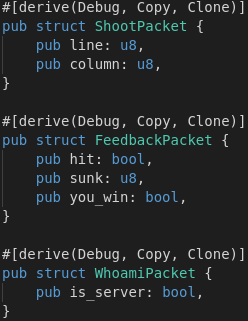
\includegraphics[scale=0.5]{Bilder/packets.png}
	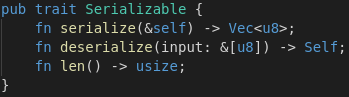
\includegraphics[scale=0.5]{Bilder/serializable.png}
\end{frame}

\begin{frame}
	\frametitle{Demo}
	\begin{center}
		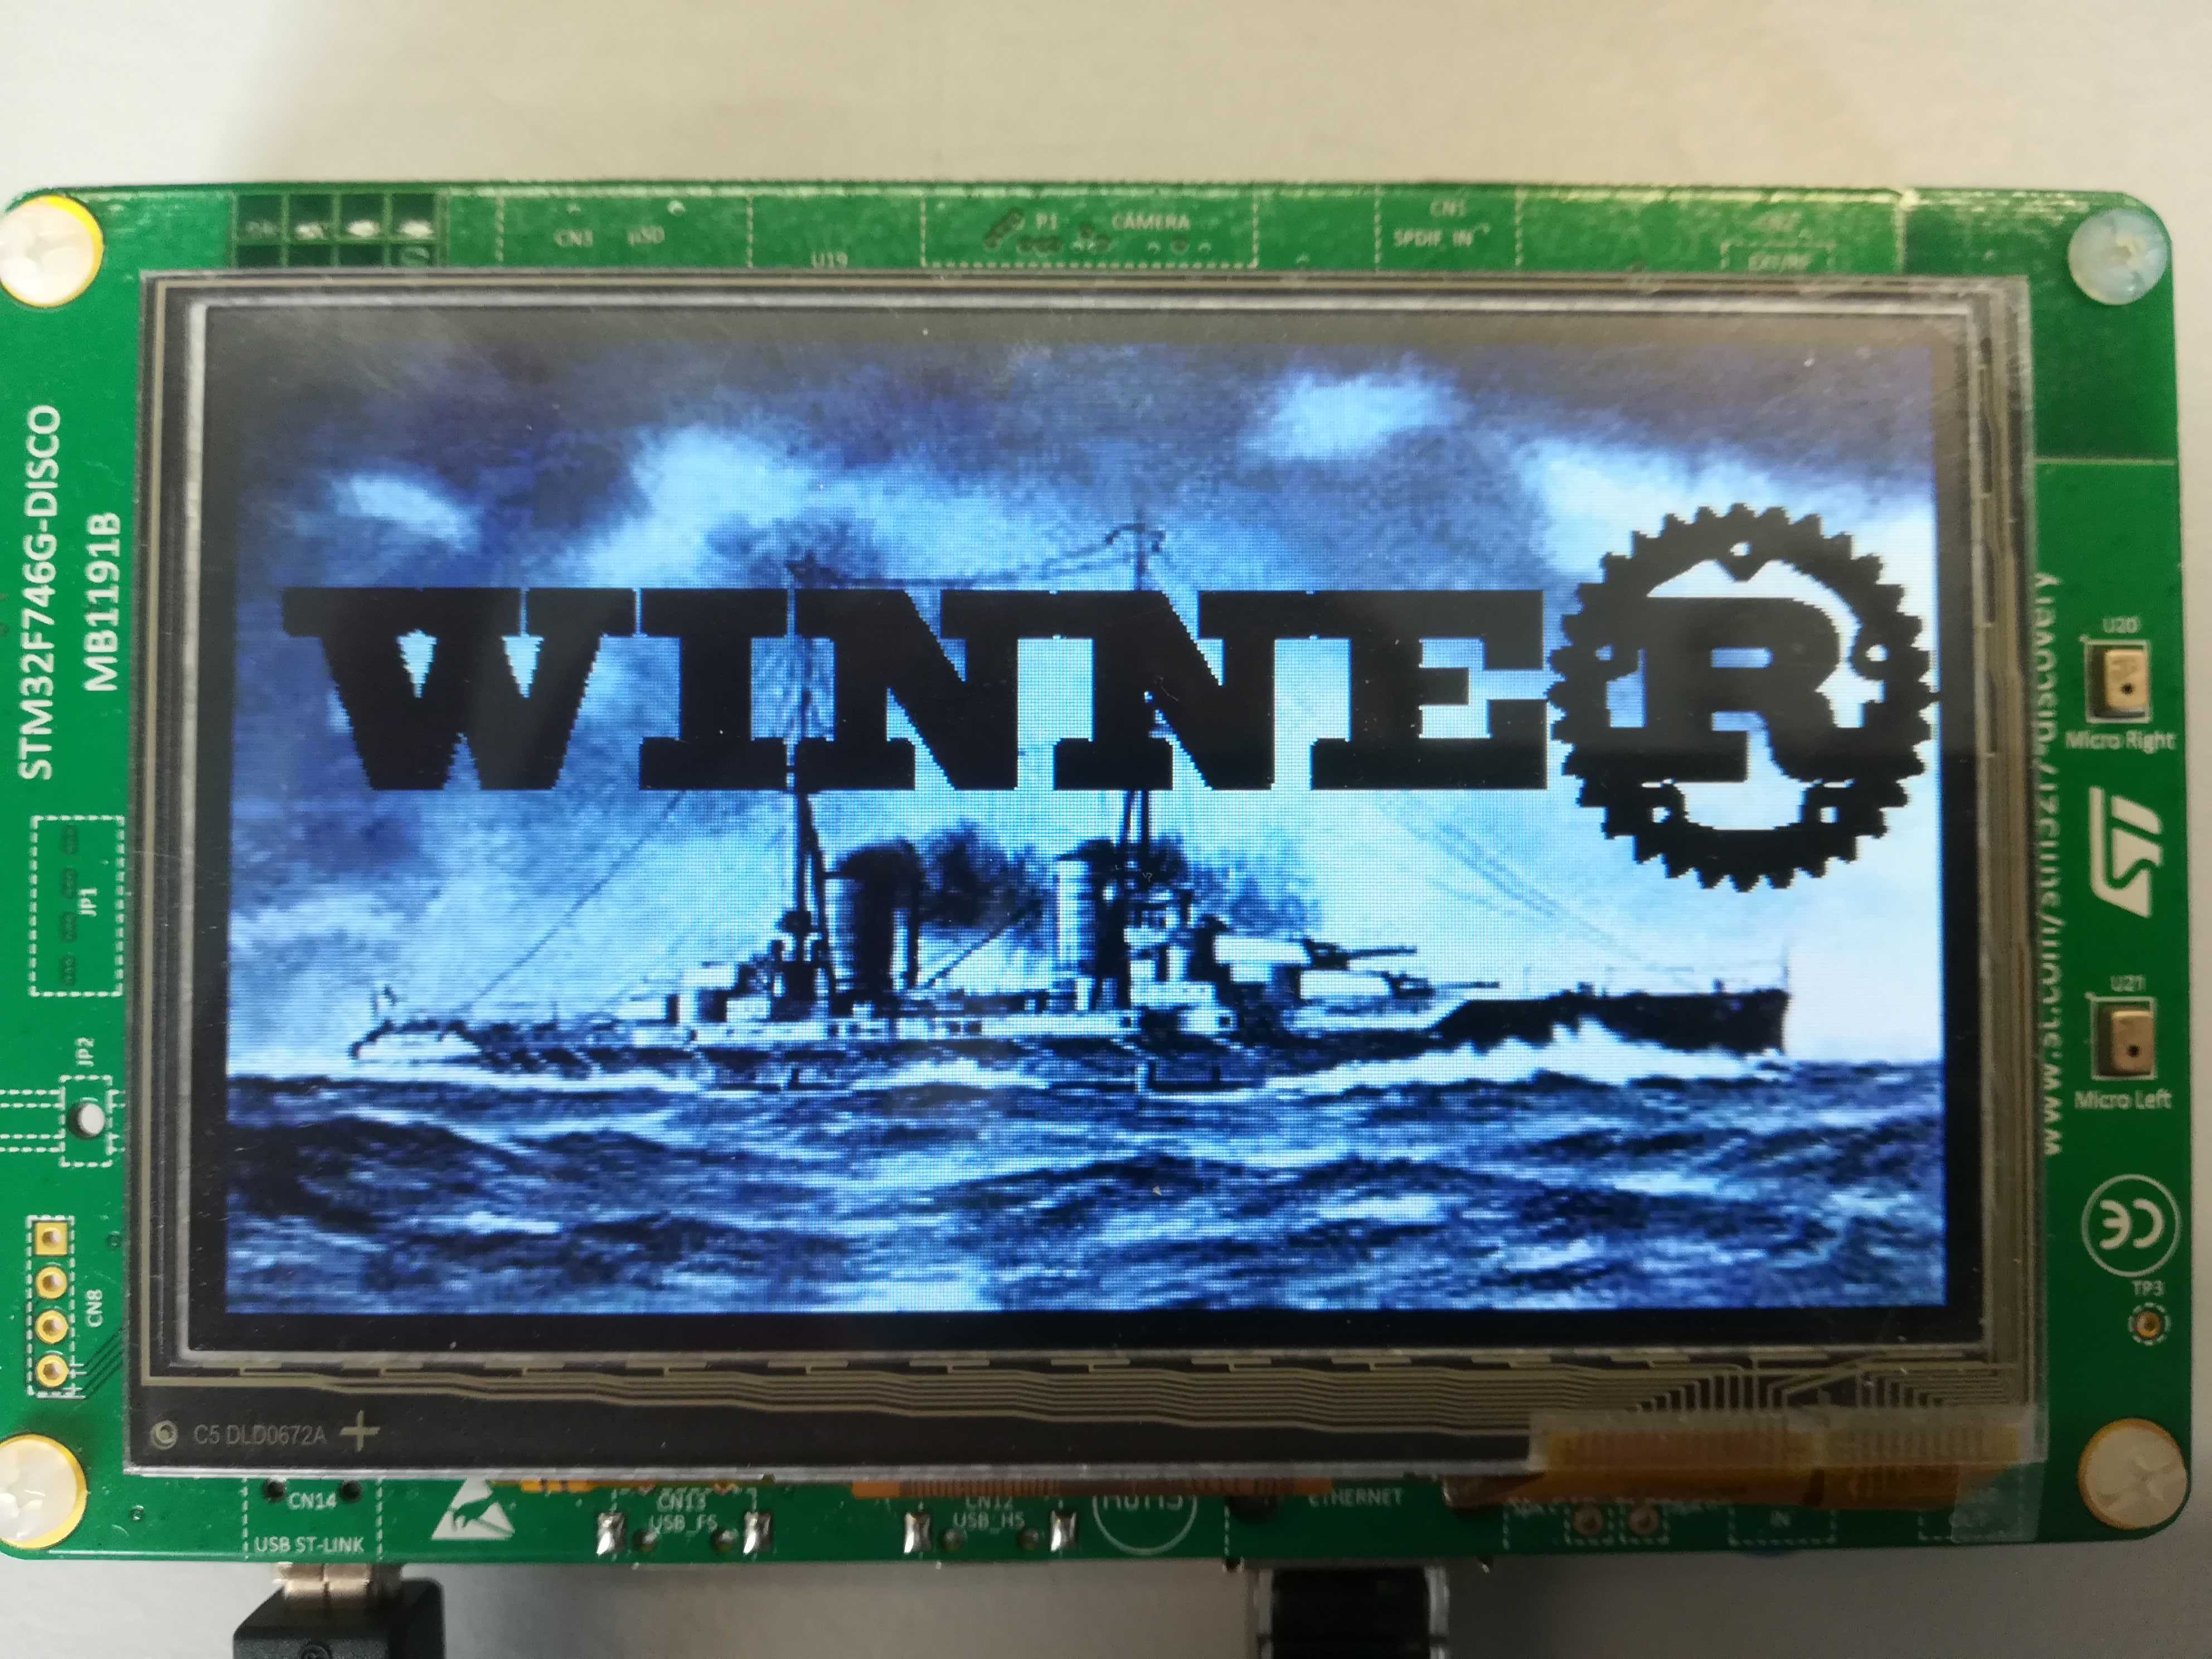
\includegraphics[scale=0.035]{Bilder/win.jpg}
		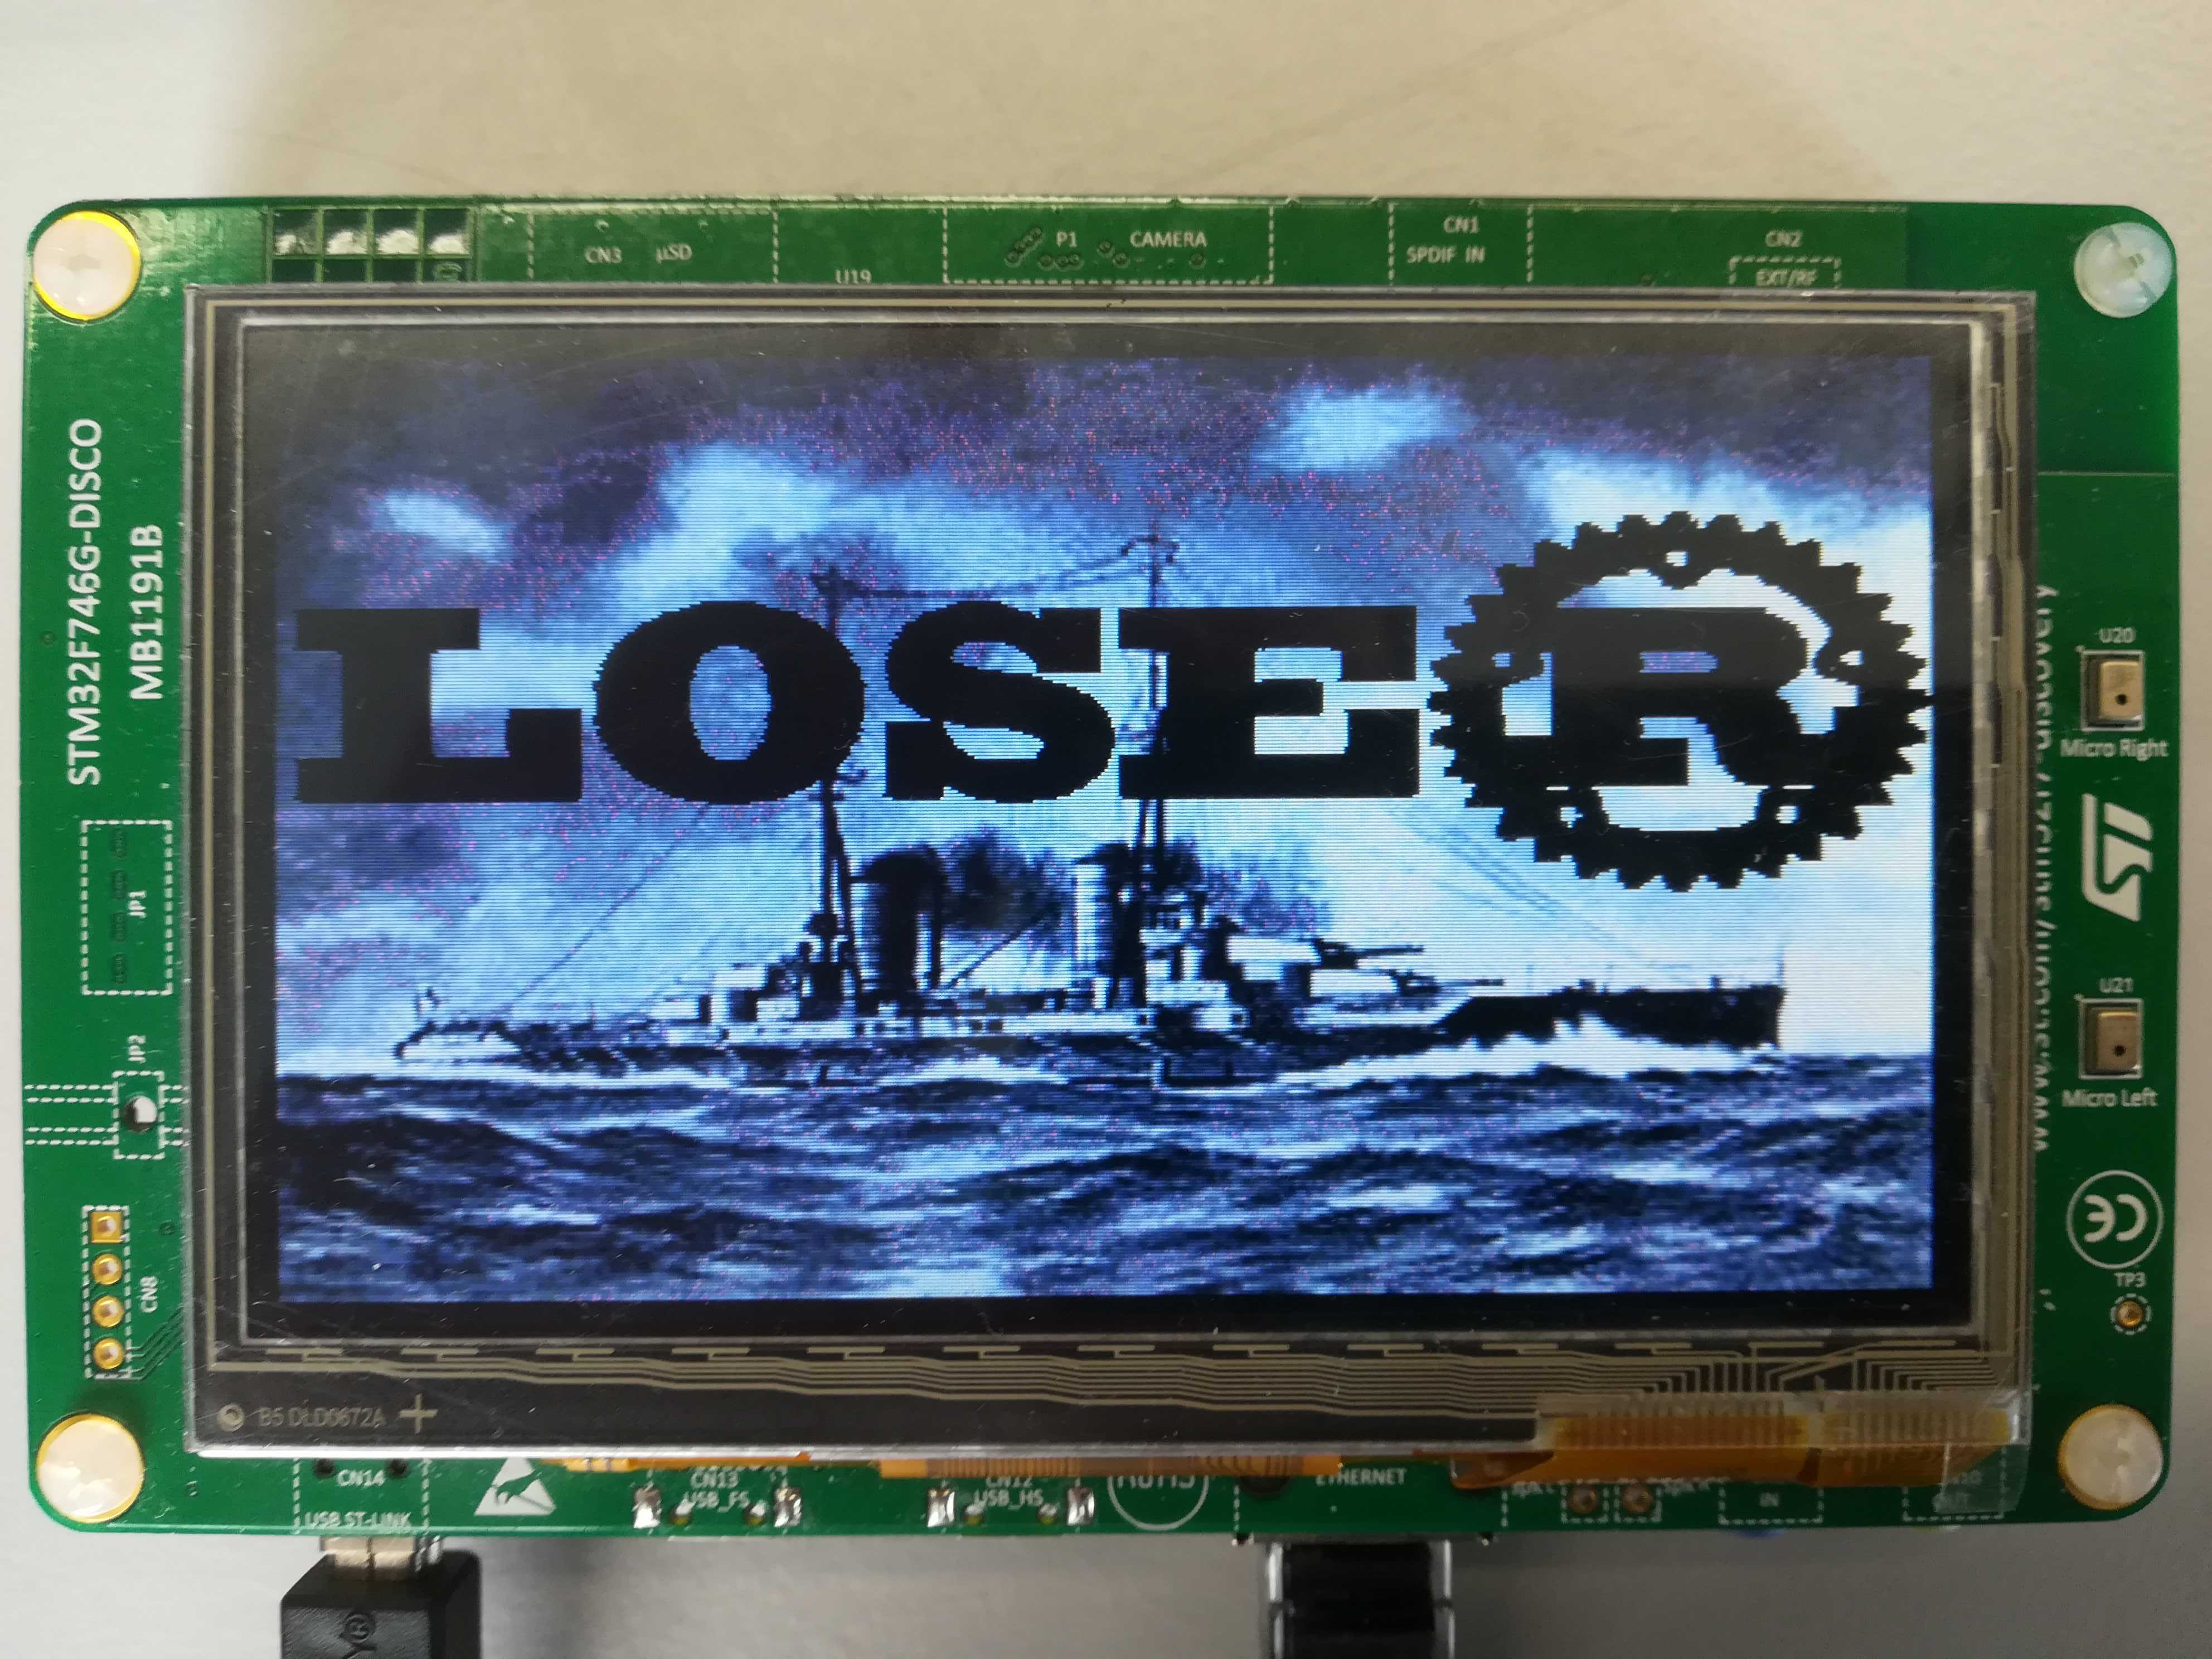
\includegraphics[scale=0.035]{Bilder/lose.jpg}
	\end{center}
\end{frame}

\begin{frame}
	\frametitle{The End}
	\begin{center}
	\Huge Thank you for your attention!
	\end{center}
\end{frame}

\end{document}
